\documentclass[conference]{IEEEtran}
\usepackage{cite}
\usepackage{graphicx}
\usepackage{amsmath,amssymb,amsfonts}
\usepackage{textcomp}
\usepackage{url}
\usepackage[hidelinks]{hyperref}
\usepackage{xcolor}
\emergencystretch=3em
\setcounter{dbltopnumber}{2}
\renewcommand{\dbltopfraction}{0.95}
\renewcommand{\dblfloatpagefraction}{0.85}
\renewcommand{\textfraction}{0.05}
\newcommand{\CADDAM}{CADD\allowbreak{}+\allowbreak{}AlphaMissense}
\newcommand{\GCNCADDAM}{GCN\allowbreak{}+\allowbreak{}CADD\allowbreak{}+\allowbreak{}AlphaMissense}

\title{Auditing PPI Graph Augmentation for Missense Variant Pathogenicity Prediction under Topology, Connectivity and Homology Constraints}

\author{}
\hypersetup{pdfauthor={}}

\begin{document}
\maketitle


\begin{abstract}
\bfseries\boldmath
We audit whether fixed two-hop protein-feature propagation (FPP) improves missense variant pathogenicity prediction on 177,213 ClinVar variants and one STRING functional-association network. FPP has no learned graph parameters. Under matched training conditions, mean AUC increased from 0.7835 for raw protein embeddings to 0.7950 for FPP, but protein-clustered uncertainty included zero gain. Connectivity and topology-permutation controls showed sensitivity to graph construction and protein--topology correspondence. With CADD and AlphaMissense, FPP improved over raw-embedding fusion, while its advantage over edge-ablated fusion remained uncertain. Under homology-aware splitting, repeated fusion runs established neither benefit nor consistent harm over the score baseline. Topology profiles and prediction changes remain exploratory. These findings support matched controls and split-aware uncertainty; they do not establish limits on trained graph models or generalize beyond this dataset and network.

\end{abstract}

\begin{IEEEkeywords}
\bfseries\boldmath
Missense variant pathogenicity, STRING networks, fixed feature propagation, protein language models, evaluation audit.
\end{IEEEkeywords}

\section{Introduction}

Missense variant pathogenicity prediction has been advanced by established methods such as CADD, REVEL, MVP, PrimateAI, EVE and AlphaMissense \cite{Kircher2014CADD,Ioannidis2016REVEL,Qi2021MVP,Sundaram2018PrimateAI,Frazer2021EVE,Cheng2023AlphaMissense}, as well as by protein language models such as ESM \cite{Lin2023ESM}. These approaches capture sequence, evolutionary and annotation-derived signals. Disease-associated proteins are also embedded in molecular interaction networks, and disease-associated mutations can perturb protein-protein and other macromolecular interactions \cite{Barabasi2011NetworkMedicine,Menche2015DiseaseModules,Sahni2015InteractionPerturbation,Chen2018InteractomePerturbation}. PPI graphs provide an additional source of context for missense variant prediction.

Earlier approaches incorporated protein-interaction and other molecular-network features into single-amino-acid variant prioritization, showing that network context can provide information complementary to sequence, structure and annotation features \cite{Yates2014SuSPect,Ozturk2022NetworkFeatures}. More recent graph-based variant predictors include graph attention models for missense effects, heterogeneous gene-variant graph approaches, multimodal variant graph methods and disease-specific graph models \cite{Zhang2022gMVP,Cheng2021VEGN,Yu2025GNNMAP,Ghadie2025DiseaseSpecificGNN}. These studies establish the relevance of relational structure to variant interpretation. We focus on how to interpret gains obtained by propagating protein language model embeddings over a shared STRING association graph before variant-level classification.

A shared-graph setting mixes several effects. Train, validation and test variants may have distinct protein identifiers while their proteins remain directly connected in the same STRING graph. Related proteins may also cross partitions when homology is not explicitly controlled \cite{Littmann2022ProteinMLTips,Teufel2023GraphPart}. Strong variant-effect predictors such as CADD and AlphaMissense can further reduce the marginal contribution of graph propagation. We evaluate protein-topology correspondence, graph connectivity, protein-level uncertainty, homology-aware performance and complementarity to established predictors.

We audit raw ESM, fixed propagation, external scores and fusion models on a reconstructed ClinVar-STRING dataset. The contribution is an evaluation study: it combines graph-intervention controls with capacity-matched fusion and protein-clustered uncertainty, documents sensitivities to split and comparison protocol, and describes exploratory topology and error-transition profiles. The audit does not introduce a new predictor or cover trained message-passing architectures.

\section{Materials and Methods}

\subsection{Dataset and graph construction}

ClinVar variant annotations were obtained from the official NCBI ClinVar FTP tab-delimited variant-summary file \cite{Landrum2020ClinVar}. We used the ClinVar variant-summary release dated 31 March 2024 and retained checksums for the exact input file used in the reconstruction. We reconstructed a filtered, non-conflicting missense dataset and mapped variants to STRING human protein identifiers. We retained GRCh38 germline missense SNVs with criteria-supported review status, combined pathogenic and likely pathogenic records into the positive class, combined benign and likely benign records into the negative class, removed uncertain or conflicting records, and collapsed duplicate VariationIDs. The final ClinVar-STRING dataset contained 177,213 missense variants mapped to 14,123 labelled STRING proteins. The propagation graph contained 19,622 STRING protein nodes and 13,715,404 directed edge-index entries from the STRING v12 protein-association network \cite{Szklarczyk2023STRING}. We used this network as STRING network context; its association evidence extends beyond direct physical interactions.

\subsection{Protein representations and fixed propagation}

Raw protein features were generated using the ESM-2 650M checkpoint, with 1,280-dimensional protein-level vectors obtained by residue averaging \cite{Lin2023ESM}. Fixed protein-feature propagation (FPP) was computed by two-hop GCN-style propagation over the normalized STRING graph \cite{Kipf2017GCN}. FPP has no learned graph-convolution parameters; the downstream MLP alone was trained. Fixed propagation isolates topology-induced smoothing from capacity gains due to trainable graph layers and provides a controlled representation for the audit. Let $X$ denote the raw ESM protein-representation matrix. The matched implementation adds self-loops before symmetrizing the retained edge list and sums duplicate contributions when coalescing. Thus $\tilde{A}=(E+I)+(E+I)^{\mathrm{T}}$, where $E$ is the edge-index count matrix; STRING combined scores are not propagation weights. Let $\tilde{D}$ denote its weighted degree matrix. We computed the symmetrically normalized adjacency matrix as
\begin{equation}
\hat{A}=\tilde{D}^{-\frac{1}{2}}\tilde{A}\tilde{D}^{-\frac{1}{2}},
\end{equation}
\begin{equation}
H=\frac{1}{3}\left(X+\hat{A}X+\hat{A}^{2}X\right).
\end{equation}
The fixed two-hop FPP representation $H$ averages the original ESM features, one-hop and two-hop STRING-smoothed features. Propagation used only graph structure and ESM features; downstream classification used the representation of each variant's mapped STRING protein. The full graph contained train, validation and test nodes with their ESM features, making the evaluation transductive. Held-out features and graph structure were available during propagation, but held-out labels were not used. Embedding-only models assign identical inputs to variants mapped to the same protein; they cannot resolve residue-specific effects within that protein.

\subsection{Splits, classifiers and external predictors}

The original split assigned train, validation and test variants by STRING protein ID, with no shared proteins across partitions. The split contained 141,864 training variants, 17,129 validation variants and 18,220 test variants. The homology-aware split used MMseqs-derived protein clusters, assigned each cluster wholly to one partition by greedy balancing of variant-row counts, without label-prevalence stratification, and preserved the same row counts \cite{Steinegger2017MMseqs2}. We use this split as a stress test. Its test positive rate was 10.56\%, compared with 31.95\% in the original split, which limits direct cross-split AUPRC comparison.

All current comparisons used downstream MLPs with 512/128 hidden units, dropout 0.3, Adam optimization and validation-AUC checkpoint selection \cite{Kingma2015Adam}. Classifier seeds 42--44, a maximum of 50 epochs and patience five were shared across arms; permutation controls crossed three graph permutations with the same classifier seeds. CADD v1.7 and AlphaMissense scores were matched to variant records \cite{Schubach2024CADDv17,Cheng2023AlphaMissense}. Missing values were imputed using training-set medians, with an AlphaMissense missingness indicator; inputs were not standardized. Models shared hidden layers and preprocessing, although score-only models had fewer input weights. Training hyperparameters, score coverage and historical protocols are detailed in Supplementary Methods 3 and 5 and Tables 1 and 8.

\subsection{Audit analyses}

Uncertainty was assessed using variant-level bootstrap and protein-clustered bootstrap \cite{Efron1993Bootstrap}. Connectivity tests removed direct train-test STRING edges and regenerated FPP embeddings. Partial edge-ablation curves removed 0\%, 25\%, 50\%, 75\% and 100\% of direct train-test protein pairs using random removal, higher-STRING-score-first removal and lower-STRING-score-first removal. Topology permutation preserved the unlabeled graph structure and randomized the correspondence between protein identity and graph position, testing whether generic graph smoothing explained the gain. Fusion controls concatenated \CADDAM{} features with raw ESM, edge-ablated FPP and topology-permuted FPP representations, testing representation complementarity and sensitivity to protein-topology correspondence. Edge removal also changes normalization and retains indirect cross-partition paths; it does not isolate a causal contribution of direct connectivity.

The implementation audit identified a self-loop convention mismatch between historical full FPP and its graph controls. Current graph controls were regenerated with the full-FPP operator; the saved full-FPP representation was numerically checked. Historical controls remain separately labeled; environment restoration and numerical verification are documented in Supplementary Methods 5.

Exploratory analyses stratified retained-reference predictions by degree, k-core, betweenness, clustering and neighbour-risk features, and examined corrected and degraded predictions. Neighbour-risk features used training labels only. Feature-wise comparisons used false-discovery-rate correction \cite{Benjamini1995FDR}, but selected subgroup intervals did not account for test-set selection. AUPRC was interpreted within each split because precision-recall metrics depend on class prevalence \cite{Saito2015PrecisionRecall}.

\begin{table}[t]
\caption{Run provenance for the main results. Historical and matched protocols are in Supplementary Tables 8 and 11. Runs count fitted classifiers, not bootstrap resamples.}
\label{tab:run_sources}
\centering
\footnotesize
\setlength{\tabcolsep}{3pt}
\renewcommand{\arraystretch}{1.12}
\begin{tabular}{p{0.40\columnwidth}p{0.14\columnwidth}p{0.36\columnwidth}}
\hline
Evidence & Runs & Summary used \\
\hline
Fig. 1B,D/F representations & 3/arm & Matched seeds/operator/budget \\
Fig. 1C uncertainty & Ensemble & Paired variant/protein bootstrap \\
Fig. 1E partial ablation & Historical & Unequal protocols; descriptive \\
Fig. 2B fusion controls & 3/arm & Matched seeds/operator/budget \\
Fig. 2C fusion intervals & Ensemble & Protein-clustered bootstrap \\
Fig. 2E homology fusion & 3/arm & Matched score/raw/FPP arms \\
Fig. 2D; Fig. 3 & 1/arm & Historical retained predictions \\
\hline
\end{tabular}
\par\smallskip
\raggedright Each permutation arm uses 3 graphs by 3 classifier seeds (9 fits). All 48 new fits allow at most 50 epochs. Bootstrap intervals condition on fitted predictions; permutations are not 9 independent graph samples. Historical error transitions appear in Supplementary Fig. S1.
\end{table}

\section{Results}

\subsection{Full-graph FPP gains and connectivity sensitivity}

Table~\ref{tab:run_sources} separates new matched fits from historical retained predictions. With classifier seeds 42--44, raw ESM reached test AUC 0.7835 $\pm$ 0.0063 and AUPRC 0.6116 $\pm$ 0.0066; full FPP reached AUC 0.7950 $\pm$ 0.0016 and AUPRC 0.6484 $\pm$ 0.0118 (Fig. 1B). On ensemble-averaged predictions, the FPP-minus-ESM AUC difference was +0.0107, with protein-clustered 95\% CI [-0.0218, +0.0426]; the AUPRC difference was +0.0413, CI [-0.0109, +0.0770] (Fig. 1C). Variant resampling ignores within-protein dependence and gives a different uncertainty estimate. These intervals condition on the three fitted classifiers, rather than incorporating retraining variability.

Removing 1,242,422 direct train-test edge-index entries (9.06\%; 621,211 unique undirected pairs) and recomputing the same normalized operator gave edge-ablated FPP AUC 0.7702 $\pm$ 0.0077 and AUPRC 0.6075 $\pm$ 0.0139 (Fig. 1D). Repeating with three topology permutations by the same three classifier seeds gave pooled AUC 0.7803 $\pm$ 0.0092 and AUPRC 0.6102 $\pm$ 0.0085 (Fig. 1F). Per-graph and paired-seed results are retained separately in Supplementary Table 11. Matched protocols remove the previous seed, budget and self-loop mismatches, but edge removal still changes degrees and indirect connectivity remains; the contrast does not identify a purely causal contribution of direct paths.

The historical partial-ablation curve (Fig. 1E) used different classifier seeds and budgets, with reused endpoints and the old control operator. It remains an exploratory dose-response description, not part of the new matched effect estimate.

\begin{figure*}[!t]
\centering
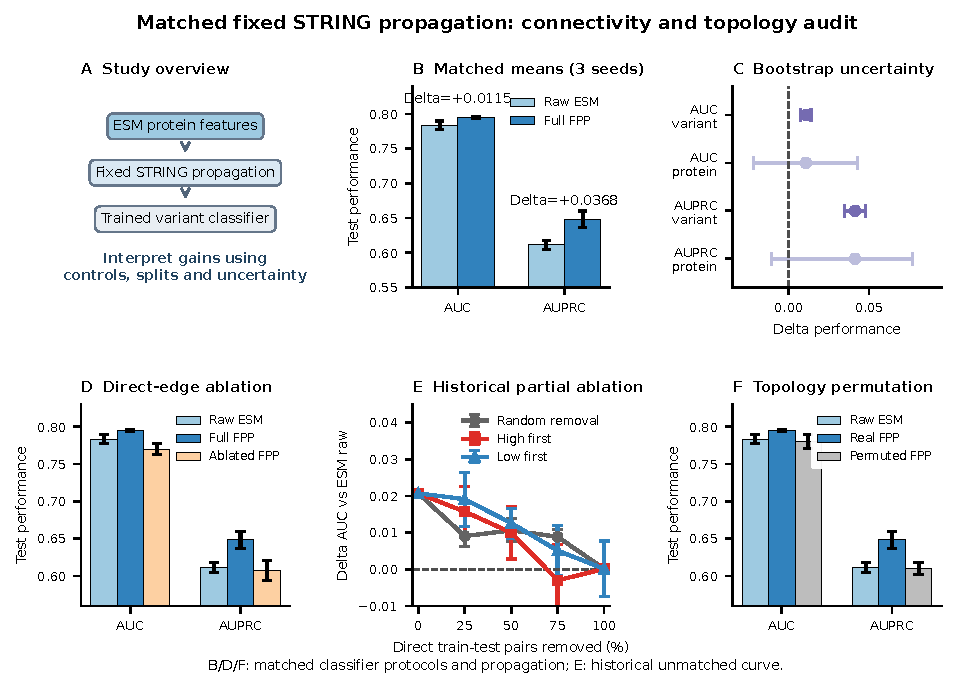
\includegraphics[width=0.98\textwidth]{figure_drafts/Figure1_fixed_propagation_audit.pdf}
\caption{Matched audit of fixed STRING propagation. A, Study overview. B, Raw ESM and full FPP: three classifier seeds per arm, mean and SD. C, Paired bootstrap of ensemble-averaged predictions, comparing variant and protein resampling; 2,000 replicates each. D, Direct-edge ablation with the common propagation operator and matched classifier protocol, mean and SD across three seeds. E, Historical partial-ablation curve with unmatched protocols and reused endpoints; it is not a matched continuation of panel D. F, Three topology permutations by the same three classifier seeds; pooled mean and SD describe both sources of dispersion. New arms share maximum 50 epochs and validation-based early stopping.}
\label{fig:connectivity}
\end{figure*}

\subsection{Architecture-matched fusion and homology-aware stress test}

On the original split, mean AUC was 0.9572 for \CADDAM{}, 0.9682 with raw embeddings and 0.9716 with FPP (Fig. 2B). The ensemble FPP-minus-raw fusion margin had a protein-clustered 95\% interval of [+0.0008, +0.0061]. The edge-ablated margin remained uncertain, whereas the permutation margin was small and positive conditional on the sampled graphs (Fig. 2C; Supplementary Table 12). These exploratory intervals are not adjusted for multiple comparisons and condition on fitted models; an interval spanning zero does not establish equivalence.

Figure 2D retains historical homology-aware representation estimates. The current homology-aware fusion comparison gave mean AUC 0.9755 for \CADDAM{}, 0.9727 with raw embeddings and 0.9752 with FPP, using three matched seeds per arm (Fig. 2E). The ensemble FPP-minus-score AUC difference was +0.0001, with protein-clustered 95\% CI [-0.0019, +0.0021]; the AUPRC interval also spanned zero (Supplementary Table 12). Thus, repeated fitting establishes neither benefit nor consistent harm from FPP relative to scores alone. Mean run metrics and metrics of averaged probabilities can give different close rankings. Redundant high-dimensional inputs, additional input weights, lack of feature scaling and altered protein composition could contribute to this behavior; these explanations were not experimentally separated. AUPRC comparisons remain within-split because prevalence differs.

\begin{figure*}[!t]
\centering
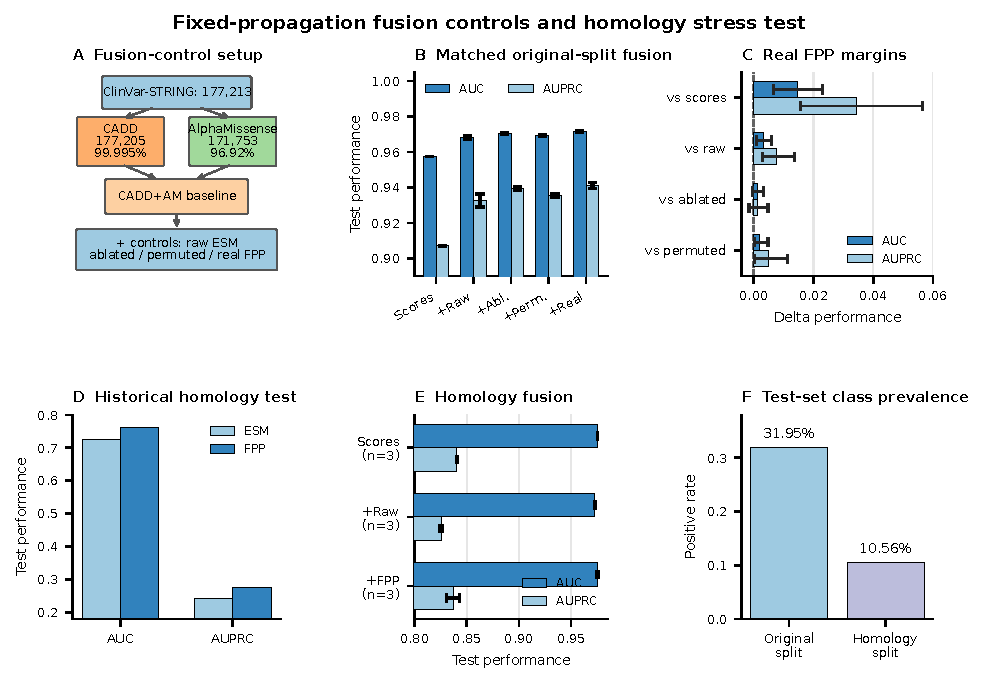
\includegraphics[width=0.98\textwidth]{figure_drafts/Figure2_fusion_homology.pdf}
\caption{Matched fusion and homology-aware evaluation. A, External-score coverage and fusion setup. B, Original-split matched fusion, mean and SD over three seeds per arm; permutation uses three graphs by three seeds. C, Real-FPP minus control performance on ensemble-averaged probabilities, with paired protein-clustered 95\% bootstrap intervals (2,000 replicates). Ensemble point differences can differ from differences of mean run metrics in B. Intervals condition on fitted models and sampled graph permutations; they omit retraining and new-permutation uncertainty. D, Historical retained homology-aware representation estimates. E, New homology-aware fusion: all three arms use the same three seeds, classifier protocol and maximum 50 epochs; error bars indicate SD. F, Test prevalence by split. Scores denotes CADD+AlphaMissense; Raw, Abl., Perm. and Real denote added representations.}
\label{fig:fusion_homology}
\end{figure*}

\subsection{Exploratory topology-context descriptions}

ESM representations showed weak correspondence with STRING topology before propagation (Fig. 3A). Historical retained-reference predictions showed non-monotonic variation across degree, k-core and other network strata (Fig. 3B--D; Supplementary Table 5). These patterns are descriptive and do not identify biological contexts that will reliably benefit on new data.

All 53 joint cells and highlighted profiles were inspected on the same test set (Fig. 3E,F). Their intervals quantify within-cell resampling, not subgroup-selection uncertainty; feature-level FDR correction does not remove this selection effect. The profiles therefore generate hypotheses for independent validation.

\begin{figure*}[!t]
\centering
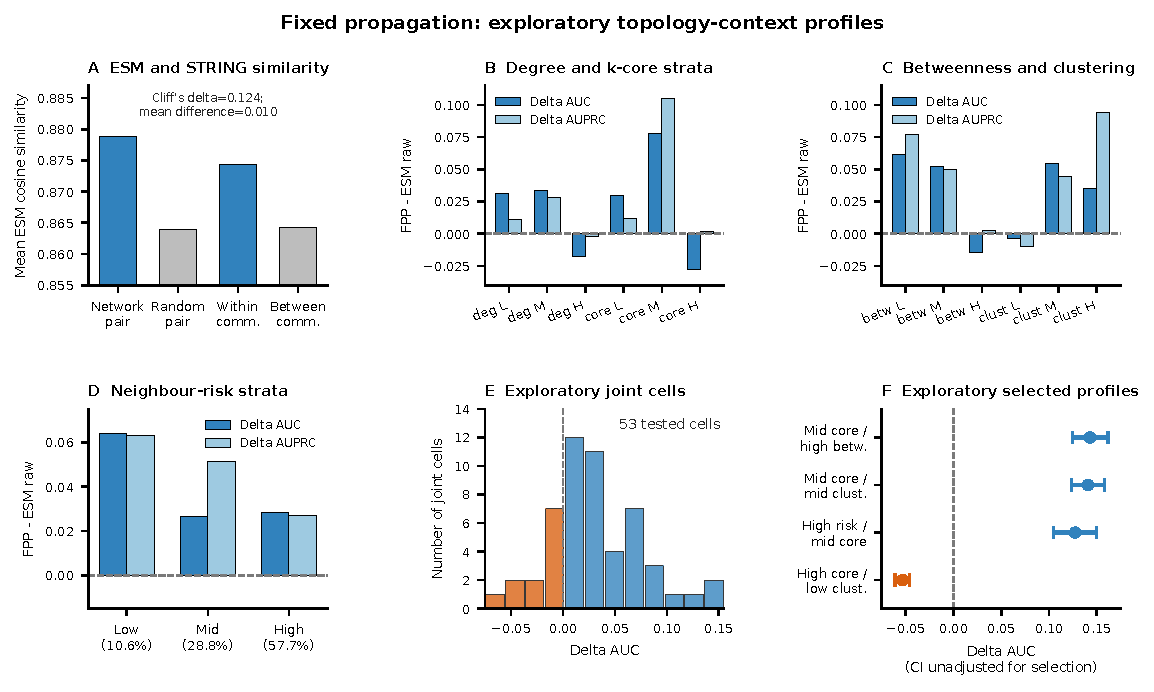
\includegraphics[width=0.98\textwidth]{figure_drafts/Figure3_exploratory_topology.pdf}
\caption{Exploratory descriptions of retained-reference FPP gains across network topology contexts. A, ESM representations show weak alignment with STRING topology. B, Degree and k-core gains are non-monotonic. C-D, Stratified estimates differ across betweenness, clustering and neighbour-risk groups. E, Exploratory joint-cell distribution. L/M/H denote low/mid/high strata; deg, core, betw and clust denote degree, k-core, betweenness and clustering. F, Exploratory selected profiles; intervals are unadjusted for test-set selection and require independent validation.}
\label{fig:topology_context}
\end{figure*}

Historical retained prediction pairs also showed both corrected and degraded variants after adding graph context. Their error-type balance changed with the decision threshold, and the class-weighted scores were uncalibrated. These exploratory transitions are reported in Supplementary Tables 6 and 10 and Figure S1.

\section{Discussion}

Matched comparisons support an evaluation-dependent effect of fixed propagation. Mean performance improved over raw embeddings, but protein-level intervals for that gain crossed zero. Graph interventions show sensitivity to connectivity and protein--topology correspondence; edge removal also changes normalization and leaves indirect paths, so it does not isolate a causal connectivity effect. The transductive design permits held-out protein features and graph structure, without held-out labels.

The homology-aware fusion results do not support a claim of consistent graph-induced deterioration. Three matched seeds resolve the previous unequal repeat count, while uncertainty remains around the graph-versus-score comparison. Redundant high-dimensional features and changes in protein composition offer plausible explanations, rather than established mechanisms. The frozen partition and differing prevalence limit broader cross-split conclusions.

Generalization remains limited to one reconstructed ClinVar cohort and one STRING functional-association network, which includes associations beyond physical interactions \cite{Szklarczyk2023STRING}. No independent cohort or second network was tested, and overlap with the development data of external predictors was not excluded. Fixed propagation does not establish what learned graph models could achieve. Selected topology profiles and uncalibrated prediction transitions require independent confirmation. Further methodological boundaries and sensitivity analyses are retained in the supplement.

\paragraph{Practical recommendations}
Compare graph features with both raw protein embeddings and strong score baselines. Use the same training protocol across controls and report whether held-out proteins are visible in the graph. Quantify uncertainty at the protein level and check gains within the intended split. Treat selected subgroups as hypotheses, and evaluate calibration before using prediction changes to guide decisions.

\section{Conclusion}
Fixed STRING propagation shows evaluation-dependent gains on this ClinVar cohort. Graph controls and strong baselines are essential to interpret those gains. The present evidence neither establishes a performance ceiling nor determines how trained graph models or independent cohorts would behave.

\section*{Data and Code Availability}

Code, dated manuscript revisions and matched-experiment records are publicly archived; the identifying repository URL is withheld in this anonymous copy. The archive includes environment specifications, per-run metrics, predictions and input checksums. Large provider resources and training tensors are not redistributed; reconstruction uses resources obtained from ClinVar, STRING, CADD and AlphaMissense.

\section*{AI-Tool Disclosure}

OpenAI ChatGPT, OpenAI Codex and Anthropic Claude supported literature organization, analysis-code drafting and language editing. Historical experiments were performed by the authors. Revision-stage scripts assisted by these tools restored an isolated runtime, checked input provenance, trained matched downstream classifiers on the provided data, and recomputed sensitivity statistics. Actual logs, fitted predictions and checksums are retained for review. The authors retain responsibility for study design, interpretation, citation verification and final approval. The tools are not authors; no synthetic outcomes were substituted for experimental results.

\begin{thebibliography}{99}
\bibitem{Barabasi2011NetworkMedicine} A.-L. Barabasi, N. Gulbahce, and J. Loscalzo, ``Network medicine: a network-based approach to human disease,'' \emph{Nature Reviews Genetics}, vol. 12, pp. 56--68, 2011, doi: 10.1038/nrg2918.
\bibitem{Benjamini1995FDR} Y. Benjamini and Y. Hochberg, ``Controlling the false discovery rate: a practical and powerful approach to multiple testing,'' \emph{Journal of the Royal Statistical Society: Series B}, vol. 57, pp. 289--300, 1995, doi: 10.1111/j.2517-6161.1995.tb02031.x.
\bibitem{Chen2018InteractomePerturbation} S. Chen et al., ``An interactome perturbation framework prioritizes damaging missense mutations for developmental disorders,'' \emph{Nature Genetics}, vol. 50, pp. 1032--1040, 2018, doi: 10.1038/s41588-018-0130-z.
\bibitem{Cheng2021VEGN} J. Cheng, C. Lawrence, and M. Niepert, ``VEGN: variant effect prediction with graph neural networks,'' arXiv:2106.13642, 2021, doi: 10.48550/arXiv.2106.13642.
\bibitem{Cheng2023AlphaMissense} J. Cheng et al., ``Accurate proteome-wide missense variant effect prediction with AlphaMissense,'' \emph{Science}, vol. 381, eadg7492, 2023, doi: 10.1126/science.adg7492.
\bibitem{Efron1993Bootstrap} B. Efron and R. J. Tibshirani, \emph{An Introduction to the Bootstrap}. Chapman \& Hall/CRC, 1993.
\bibitem{Frazer2021EVE} J. Frazer et al., ``Disease variant prediction with deep generative models of evolutionary data,'' \emph{Nature}, vol. 599, pp. 91--95, 2021, doi: 10.1038/s41586-021-04043-8.
\bibitem{Ghadie2025DiseaseSpecificGNN} M. Ghadie, S. Sardaar, and Y. Trakadis, ``Disease-specific prediction of missense variant pathogenicity with DNA language models and graph neural networks,'' \emph{Bioengineering}, vol. 12, p. 1098, 2025, doi: 10.3390/bioengineering12101098.
\bibitem{Ioannidis2016REVEL} N. M. Ioannidis et al., ``REVEL: an ensemble method for predicting the pathogenicity of rare missense variants,'' \emph{American Journal of Human Genetics}, vol. 99, pp. 877--885, 2016, doi: 10.1016/j.ajhg.2016.08.016.
\bibitem{Kingma2015Adam} D. P. Kingma and J. Ba, ``Adam: a method for stochastic optimization,'' \emph{International Conference on Learning Representations}, 2015, arXiv:1412.6980.
\bibitem{Kipf2017GCN} T. N. Kipf and M. Welling, ``Semi-supervised classification with graph convolutional networks,'' \emph{International Conference on Learning Representations}, 2017.
\bibitem{Kircher2014CADD} M. Kircher et al., ``A general framework for estimating the relative pathogenicity of human genetic variants,'' \emph{Nature Genetics}, vol. 46, pp. 310--315, 2014, doi: 10.1038/ng.2892.
\bibitem{Landrum2020ClinVar} M. J. Landrum et al., ``ClinVar: improvements to accessing data,'' \emph{Nucleic Acids Research}, vol. 48, pp. D835--D844, 2020, doi: 10.1093/nar/gkz972.
\bibitem{Lin2023ESM} Z. Lin et al., ``Evolutionary-scale prediction of atomic-level protein structure with a language model,'' \emph{Science}, vol. 379, pp. 1123--1130, 2023, doi: 10.1126/science.ade2574.
\bibitem{Littmann2022ProteinMLTips} Q. Hou, K. Waury, D. Gogishvili, and K. A. Feenstra, ``Ten quick tips for sequence-based prediction of protein properties using machine learning,'' \emph{PLOS Computational Biology}, vol. 18, no. 12, Art. no. e1010669, 2022, doi: 10.1371/journal.pcbi.1010669.
\bibitem{Menche2015DiseaseModules} J. Menche et al., ``Disease networks. Uncovering disease-disease relationships through the incomplete interactome,'' \emph{Science}, vol. 347, 1257601, 2015, doi: 10.1126/science.1257601.
\bibitem{Ozturk2022NetworkFeatures} K. Ozturk and H. Carter, ``Predicting functional consequences of mutations using molecular interaction network features,'' \emph{Human Genetics}, vol. 141, pp. 1195--1210, 2022, doi: 10.1007/s00439-021-02329-5.
\bibitem{Qi2021MVP} H. Qi et al., ``MVP predicts the pathogenicity of missense variants by deep learning,'' \emph{Nature Communications}, vol. 12, p. 510, 2021, doi: 10.1038/s41467-020-20847-0.
\bibitem{Sahni2015InteractionPerturbation} N. Sahni et al., ``Widespread macromolecular interaction perturbations in human genetic disorders,'' \emph{Cell}, vol. 161, pp. 647--660, 2015, doi: 10.1016/j.cell.2015.04.013.
\bibitem{Saito2015PrecisionRecall} T. Saito and M. Rehmsmeier, ``The precision-recall plot is more informative than the ROC plot when evaluating binary classifiers on imbalanced datasets,'' \emph{PLOS ONE}, vol. 10, e0118432, 2015, doi: 10.1371/journal.pone.0118432.
\bibitem{Schubach2024CADDv17} M. Schubach et al., ``CADD v1.7: using protein language models, regulatory CNNs and other nucleotide-level scores to improve genome-wide variant predictions,'' \emph{Nucleic Acids Research}, vol. 52, no. D1, pp. D1143--D1154, 2024, doi: 10.1093/nar/gkad989.
\bibitem{Steinegger2017MMseqs2} M. Steinegger and J. Soding, ``MMseqs2 enables sensitive protein sequence searching for the analysis of massive data sets,'' \emph{Nature Biotechnology}, vol. 35, pp. 1026--1028, 2017, doi: 10.1038/nbt.3988.
\bibitem{Sundaram2018PrimateAI} L. Sundaram et al., ``Predicting the clinical impact of human mutation with deep neural networks,'' \emph{Nature Genetics}, vol. 50, pp. 1161--1170, 2018, doi: 10.1038/s41588-018-0167-z.
\bibitem{Szklarczyk2023STRING} D. Szklarczyk et al., ``The STRING database in 2023: protein-protein association networks and functional enrichment analyses for any sequenced genome of interest,'' \emph{Nucleic Acids Research}, vol. 51, pp. D638--D646, 2023, doi: 10.1093/nar/gkac1000.
\bibitem{Teufel2023GraphPart} F. Teufel, M. H. Gislason, J. J. Almagro Armenteros, A. R. Johansen, O. Winther, and H. Nielsen, ``GraphPart: homology partitioning for biological sequence analysis,'' \emph{NAR Genomics and Bioinformatics}, vol. 5, lqad088, 2023, doi: 10.1093/nargab/lqad088.
\bibitem{Yates2014SuSPect} C. M. Yates, I. Filippis, L. A. Kelley, and M. J. E. Sternberg, ``SuSPect: enhanced prediction of single amino acid variant phenotype using network features,'' \emph{Journal of Molecular Biology}, vol. 426, pp. 2692--2701, 2014, doi: 10.1016/j.jmb.2014.04.026.
\bibitem{Yu2025GNNMAP} H. Yu et al., ``A graph neural network approach for accurate prediction of pathogenicity in multi-type variants,'' \emph{Briefings in Bioinformatics}, vol. 26, bbaf151, 2025, doi: 10.1093/bib/bbaf151.
\bibitem{Zhang2022gMVP} H. Zhang, M. S. Xu, X. Fan, W. K. Chung, and Y. Shen, ``Predicting functional effect of missense variants using graph attention neural networks,'' \emph{Nature Machine Intelligence}, vol. 4, no. 11, pp. 1017--1028, 2022, doi: 10.1038/s42256-022-00561-w.
\end{thebibliography}
\end{document}
